\section{Results}\label{sec:results}

\subsection{Benchmarks}
Of the {{n_pairs}} repair events, {{real_ok}} passed the endpoint checks and {{real_one_minimal}} reached a 1-minimal repair within the probe budget; {{real_small_repair_pct}}\% of minimal repairs changed one or two line hunks. {{multi_share}}\% of the minimal repairs spanned more than one category and were excluded from the gold; the remaining {{n_real_gold}} single-mechanism items are dominated by output text (the course graded output byte for byte), followed by computation, missing statements, branch conditions, loop boundaries, output format and control flow ({{audit_control_flow_return}} of the {{audit_control_flow}} audited control-flow repairs added the \texttt{return 0} that C90 needs for a zero exit status). The controlled benchmark contains {{n_injected}} mutants over nine categories; {{injected_equivalent_pct}}\% of candidate mutants passed every test and were discarded as equivalent on the suite. Full counts are released with the benchmark (\texttt{stats.json}).

\subsection{Test signatures mix mechanisms (H1a, H1b)}
Identical test signatures often hide different mechanisms (\cref{fig:ceiling}). The best any function of the test-outcome OAV can do is to assign {{real_H1a_pct}}\% of real items (mean ceiling {{real_H1a_mean}}, 95\% CI [{{real_H1a_lo}}, {{real_H1a_hi}}]) and {{injected_H1a_pct}}\% of injected items ([{{injected_H1a_lo}}, {{injected_H1a_hi}}]) to their mechanism, so H1a is supported on both benchmarks. Put differently, {{real_collision_pct}}\% of the {{real_same_signature_pairs}} real pairs that share a test signature within an assignment have different mechanisms, and {{injected_collision_pct}}\% of the {{injected_same_signature_pairs}} injected pairs do. The refinement added by deviation OAV raises the ceiling by {{real_H1b_mean}} [{{real_H1b_lo}}, {{real_H1b_hi}}] on real and {{injected_H1b_mean}} [{{injected_H1b_lo}}, {{injected_H1b_hi}}] on injected cohorts beyond a random refinement of the same granularity (H1b supported; Holm $p={{real_H1b_p}}$ and {{injected_H1b_p}}). The extra distinctions therefore carry mechanism information rather than mere resolution.

\begin{figure}[t]
\centering
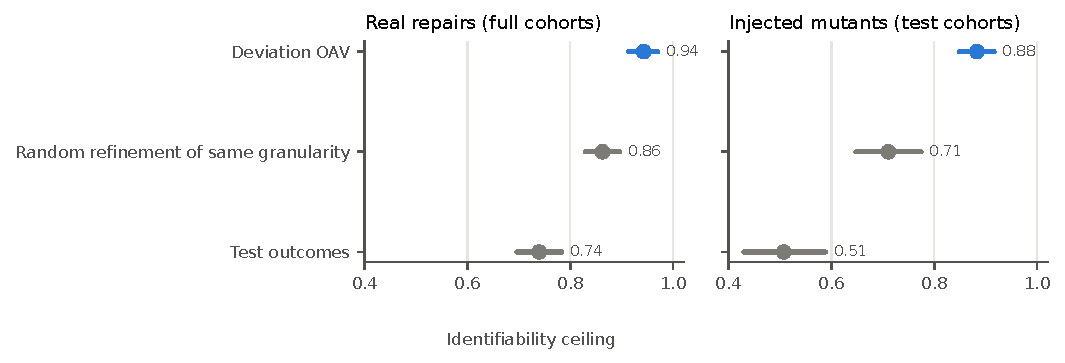
\includegraphics[width=\textwidth]{figures/ceiling_en.pdf}
\caption{Identifiability ceiling: the highest share of items that any function of a representation can assign to their mechanism. Deviation OAV exceeds both the test-outcome OAV and a random refinement with the same bucket sizes. Points are means over cohorts; bars are 95\% bootstrap intervals.}\label{fig:ceiling}
\end{figure}

\subsection{Clustering by mechanism (H2, H3)}
\Cref{tab:ari,fig:ari} report mechanism recovery at the same clustering budget. On the controlled benchmark, clusters of the test-outcome OAV barely agree with mechanisms (ARI {{injected_ari_outcomes}}, exact signatures {{injected_ari_exact}}), while deviation OAV reaches {{injected_ari_deviation}}: a difference of {{injected_H2_kmeans_mean}} [{{injected_H2_kmeans_lo}}, {{injected_H2_kmeans_hi}}] with K-means and {{injected_H2_hac_mean}} [{{injected_H2_hac_lo}}, {{injected_H2_hac_hi}}] with HAC, larger in {{injected_H2_kmeans_wins}} cohorts. On real repairs the test-outcome OAV already reaches {{real_ari_outcomes}} because the dominant output-text category produces distinctive signatures; deviation OAV reaches {{real_ari_deviation}} with K-means and {{real_arihac_deviation}} with HAC, but the differences ({{real_H2_kmeans_mean}}, CI [{{real_H2_kmeans_lo}}, {{real_H2_kmeans_hi}}]; {{real_H2_hac_mean}}, CI [{{real_H2_hac_lo}}, {{real_H2_hac_hi}}]) are not reliable. H2 is therefore supported on the controlled benchmark only and, by the registered rule, not supported overall.

H3 is not supported: evidence OAV and the earlier combined+stdout baseline are indistinguishable on both benchmarks (differences {{real_H3_kmeans_mean}} and {{injected_H3_kmeans_mean}}). Simple output relations already capture most of what distance-based clustering can exploit; outcomes+stdout reaches {{real_ari_outcomes_stdout}} and {{injected_ari_outcomes_stdout}}. Selecting $k$ by silhouette instead of the oracle lowers all scores slightly and preserves the ordering (\cref{tab:ari}).

\begin{table}[t]
\centering
\caption{Mechanism recovery on the two benchmarks: mean ARI over cohorts (oracle $k$ unless stated) and mean identifiability ceiling. Real repairs: full per-assignment cohorts (amendment A3); injected mutants: sealed test-partition cohorts.}\label{tab:ari}
\small
\begin{tabular}{lrrrr}
\toprule
Representation & K-means & HAC & K-means, silh.\ $k$ & Ceiling \\
\midrule
\multicolumn{5}{l}{\emph{Real repairs}} \\
{{table_ari_real}}
\midrule
\multicolumn{5}{l}{\emph{Injected mutants}} \\
{{table_ari_injected}}
\bottomrule
\end{tabular}
\end{table}

\begin{table}[t]
\centering
\caption{Registered hypotheses: mean difference over cohorts, 95\% bootstrap interval and verdict (H1a reports the mean outcome ceiling itself).}\label{tab:hyp}
\small
\resizebox{\textwidth}{!}{%
\begin{tabular}{lrllrll}
\toprule
 & \multicolumn{3}{c}{Real repairs} & \multicolumn{3}{c}{Injected mutants} \\
\cmidrule(lr){2-4}\cmidrule(lr){5-7}
Hypothesis & Mean & 95\% CI & Verdict & Mean & 95\% CI & Verdict \\
\midrule
{{table_hypotheses}}
\bottomrule
\end{tabular}}
\end{table}

\begin{table}[t]
\centering
\caption{IF--THEN rules predicting the mechanism of test-partition students from problem-agnostic attributes, real repairs. Abstentions count as errors in macro-F1; selective accuracy is measured on answered items.}\label{tab:rules}
\small
\resizebox{\textwidth}{!}{%
\begin{tabular}{llrrr}
\toprule
Track & Model (attributes) & Macro-F1 & Coverage & Selective acc. \\
\midrule
{{table_rules_real}}
\bottomrule
\end{tabular}}
\end{table}

\begin{figure}[t]
\centering
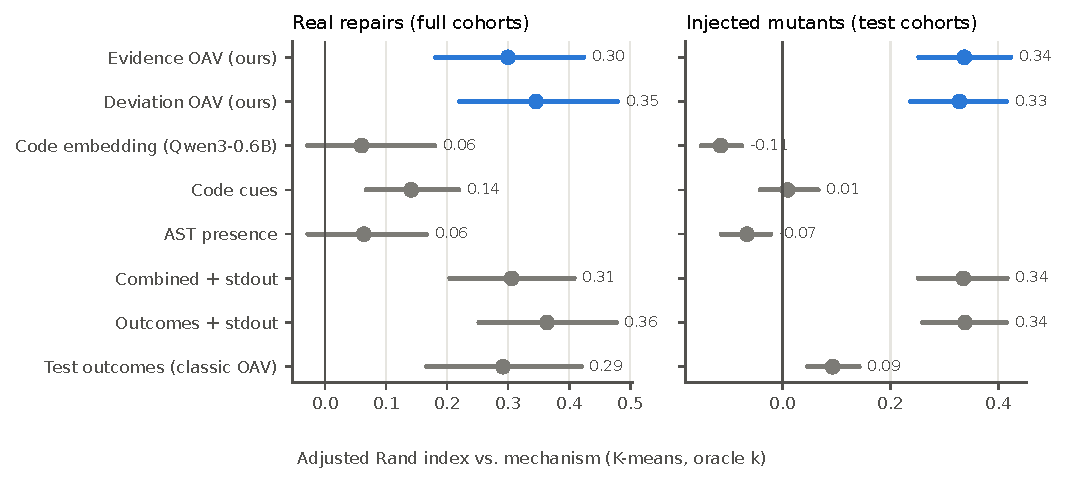
\includegraphics[width=\textwidth]{figures/ari_en.pdf}
\caption{Adjusted Rand index between clusters and mechanisms (K-means, oracle $k$). Blue: proposed representations; grey: baselines. Points are means over cohorts; bars are 95\% bootstrap intervals over cohorts.}\label{fig:ari}
\end{figure}

\subsection{Frozen code embeddings cluster programs, not mechanisms (H5)}
Qwen3-Embedding clusters of injected mutants agree more with the accepted program the mutant came from than with the injected mechanism, by {{injected_H5_mean}} ARI (95\% CI [{{injected_H5_lo}}, {{injected_H5_hi}}]; H5 supported). Their mechanism ARI is {{injected_ari_embedding}} on injected and {{real_ari_embedding}} on real cohorts. Single-token changes that decide a program's behaviour barely move a general-purpose embedding, whereas authorship and solution style dominate it.

\subsection{IF--THEN rules (H4)}
ILA-2 rules over problem-agnostic evidence attributes predicted the mechanism of real test-partition items with macro-F1 {{real_seen_problems_evidence_ila2_macro_f1}} (coverage {{real_seen_problems_evidence_ila2_coverage}}, accuracy on answered items {{real_seen_problems_evidence_ila2_selective_accuracy}}), against {{real_seen_problems_outcome_summary_ila2_macro_f1}} for rules over the outcome summary and {{real_seen_problems_majority_macro_f1}} for the majority class (\cref{tab:rules}). The difference, {{h4_mean}} [{{h4_lo}}, {{h4_hi}}], rests on the {{real_seen_problems_evidence_ila2_n}} single-mechanism items of the sealed test students and includes zero, so H4 is not supported. On the injected benchmark, where every category is represented, evidence rules reached macro-F1 {{injected_seen_problems_evidence_ila2_macro_f1}} on seen and {{injected_unseen_problems_evidence_ila2_macro_f1}} on unseen assignments, whereas outcome-summary rules reached {{injected_seen_problems_outcome_summary_ila2_macro_f1}} and {{injected_unseen_problems_outcome_summary_ila2_macro_f1}}. The noise-tolerant penalty of ILA-2 traded a little precision for much coverage: the original ILA answered {{injected_seen_problems_evidence_ila_coverage}} of injected test items with accuracy {{injected_seen_problems_evidence_ila_selective_accuracy}}, ILA-2 answered {{injected_seen_problems_evidence_ila2_coverage}} with accuracy {{injected_seen_problems_evidence_ila2_selective_accuracy}}. \Cref{tab:toprules} lists the highest-precision rules learned from real repairs; they read like the production rules of the classic formulation, but their conclusions are program-level mechanisms and their precision was measured on students not used to induce them.

\begin{table}[t]
\centering
\caption{The most precise ILA-2 rules induced from real training repairs (support: correct/matched training items).}\label{tab:toprules}
\small
\begin{tabular}{p{7.6cm}p{3.0cm}r}
\toprule
IF & THEN mechanism & Support \\
\midrule
{{table_top_rules}}
\bottomrule
\end{tabular}
\end{table}

\subsection{Which mechanisms benefit (exploratory)}
Per category (\cref{app:categories}), test signatures recover output text ({{real_rec_outcomes_output_text}}), loop boundaries ({{real_rec_outcomes_loop_boundary}}) and control flow ({{real_rec_outcomes_control_flow}}) on real repairs, but not output format ({{real_rec_outcomes_output_format}}), branch conditions ({{real_rec_outcomes_branch_condition}}) or missing statements ({{real_rec_outcomes_missing_statement}}); with deviation OAV these rise to {{real_rec_deviation_output_format}}, {{real_rec_deviation_branch_condition}} and {{real_rec_deviation_missing_statement}}. Averaged over categories, recovery rises from {{real_catrec_outcomes}} to {{real_catrec_deviation}} on real and from {{injected_catrec_outcomes}} to {{injected_catrec_deviation}} on injected cohorts. The gains of output evidence thus concentrate in the minority mechanisms that a cohort-level ARI weighs little, which explains why the real-benchmark ARI difference is small.
